%% LyX 2.0.2 created this file.  For more info, see http://www.lyx.org/.
%% Do not edit unless you really know what you are doing.
\documentclass[11pt,oneside,english]{amsbook}
\usepackage[T1]{fontenc}
\usepackage[utf8]{inputenc}
\setlength{\parskip}{\medskipamount}
\setlength{\parindent}{0pt}
\usepackage{verbatim}
\usepackage{float}
\usepackage{amsthm}
\usepackage{amssymb}
\usepackage{graphicx}
\PassOptionsToPackage{normalem}{ulem}
\usepackage{ulem}

\makeatletter

%%%%%%%%%%%%%%%%%%%%%%%%%%%%%% LyX specific LaTeX commands.
\newcommand{\noun}[1]{\textsc{#1}}
%% Because html converters don't know tabularnewline
\providecommand{\tabularnewline}{\\}
\floatstyle{ruled}
\newfloat{algorithm}{tbp}{loa}
\providecommand{\algorithmname}{Algorithm}
\floatname{algorithm}{\protect\algorithmname}

%%%%%%%%%%%%%%%%%%%%%%%%%%%%%% Textclass specific LaTeX commands.
\numberwithin{section}{chapter}
\numberwithin{equation}{section}
\numberwithin{figure}{section}
\newenvironment{lyxlist}[1]
{\begin{list}{}
{\settowidth{\labelwidth}{#1}
 \setlength{\leftmargin}{\labelwidth}
 \addtolength{\leftmargin}{\labelsep}
 \renewcommand{\makelabel}[1]{##1\hfil}}}
{\end{list}}

%%%%%%%%%%%%%%%%%%%%%%%%%%%%%% User specified LaTeX commands.
\usepackage{listings}
\usepackage{url}
\usepackage{datetime}
\usepackage{a4wide}
\usepackage{hyperref}
\usepackage{color}
\usepackage{ae,aecompl}

%\declare@shorthand{english}{""}{\hskip\z@skip}
\newcommand{\origttfamily}{}% sollte noch nicht definiert sein!
\let\origttfamily=\ttfamily % alte Definition von \ttfamily sichern
\renewcommand{\ttfamily}{\origttfamily \hyphenchar\font=`\-}
\newcommand{\lyxdot}{.}

%When using hyperref and referencing algorithms latex gives an error: ! Undefined control sequence. <argument> algorithm.\theHalgorithm This can be solved adding at the preamble:
\newcommand{\theHalgorithm}{\arabic{algorithm}}
% Some nice colors

\definecolor{royalblue}{cmyk}{.93, .79, 0, 0}
\definecolor{lightblue}{cmyk}{.10, .017, 0, 0}
\definecolor{darkgreen}{rgb}{0,.7,0}
\definecolor{darkred}{rgb}{.7,0,0}
\definecolor{gray}{gray}{0.5}
\definecolor{lightgray}{gray}{0.97}
\definecolor{forrestgreen}{cmyk}{.76, 0, .76, .45}

\lstdefinestyle{mystyle}{ 
basicstyle=\tiny\ttfamily\bfseries, 
numbers=left, 
numberstyle=\scriptsize,
stepnumber=1, 
columns=flexible,  
numbersep=15pt, mathescape,emph={function,switch,case,while,for,do,done,if,begin,end,then,else,return}, emphstyle={\color{blue}\underline\ttfamily}, emph={[2]scheme,params}, emphstyle={[2]\textit},
morecomment={[l]{//}},
morecomment={[s]{/*}{*/}},
morecomment=[l]{\%},
commentstyle=\color{forrestgreen}\ttfamily\textit, 
stringstyle=\color{gray}\ttfamily,
morestring=[b]',
} 
\lstdefinestyle{myjavastyle}{ 
language=java,
basicstyle=\tiny,
numbers=left,
stepnumber=1,
columns=flexible,
numbersep=15pt,
mathescape,
keywordstyle={\color{blue}\ttfamily},
emphstyle={\color{blue}\underline\ttfamily}, emph={[2]scheme,params}, emphstyle={[2]\textit},
morecomment={[l]{//}},
commentstyle=\color{forrestgreen}\ttfamily\textit, 
stringstyle=\color{gray}\ttfamily,
} 

\lstnewenvironment{mylstenv}[1][]{ 
	\lstset{style=mystyle, #1 }
}{}

\lstnewenvironment{myjavalstenv}[1][]{ 
	\lstset{style=myjavastyle, #1} 
}{} 

\makeatother

\usepackage{babel}

\begin{document}

\title{EvA2 Short Documentation}

\author{Fabian Becker, Marcel Kronfeld}


\dedicatory{~\\~\\~\\Dept. of Cognitive Systems, \\Prof. Dr. Andreas Zell,
\\University of Tübingen\\~\\~\\URL: \url{http://www.ra.cs.uni-tuebingen.de/software/EvA2}\\~\\~\\Last
updated: \ddmmyyyydate \today}

\maketitle
\newpage{}

\tableofcontents{}


\section*{Acknowledgements}

We like to thank all former and current developers of \noun{EvA:}
Fabian Becker, Alexander Hasel, Roland Baumann, Karsten Jung, Jürgen Wakunda, Holger
Ulmer, Felix Streichert, Christian Spieth, Hannes Planatscher, Andreas
Dräger, Michael de Paly, Marcel Kronfeld and all former students involved
in the work.

\hyphenation{Run-nable javaaddpath}

\begin{comment}
\textbackslash{}hyphenation\{Ab-stract-Op-ti-mi-za-tion-Prob-lem Ab-stract-Prob-lem-Double
Ab-stract-Prob-lem-Bi-na-ry eva2.problems\}
\end{comment}

\chapter{Introduction}

\emph{\noun{EvA2}} (an \uline{Ev}olutionary \uline{A}lgorithms
framework, revised version \uline{2}) is a comprehensive heuristic
optimization framework with emphasis on Evolutionary Algorithms implemented
in Java%
\footnote{Oracle and \emph{Java} are registered trademarks of Oracle and/or its affiliates.%
}. It is a revised version of the \noun{JavaEvA} \cite{JOptDocumentation}
optimization toolbox, which has been developed as a resumption of
the former \noun{EvA} software package \cite{Wakunda97EvA}.

\noun{EvA2} integrates several derivation free optimization methods,
preferably population based, such as Evolution Strategies, Genetic
Algorithms, Differential Evolution, Particle Swarm Optimization, as
well as classical techniques such as multi-start Hill Climbing or
Simulated Annealing.

\noun{EvA2} aims at two groups of users. Firstly, the applying user
who does not know much about the theory of Evolutionary Algorithms,
but wants to use them to solve a specific application problem. Secondly,
the scientific user who wants to investigate the performance of different
optimization algorithms or wants to compare the effect of alternative
or specialized evolutionary or heuristic operators. The latter usually
knows more about evolutionary or heuristic optimization and is able
to extend \noun{EvA2} by adding specific optimization strategies or
solution representations. Explicit usage examples for \noun{EvA2 }are
given in \cite{Kron10EvA2}.

This document is, as the title says, not an extensive manual on the
\noun{EvA2} framework, but instead a short introduction hoping to
ease access to \noun{EvA2.} Thus, the document is mainly sketched
along use-cases and tries to deliver knowledge on a top-down basis,
with most important things first and details where required. Still:
as \noun{EvA}, just as mostly any larger software package, can become
tricky sometimes, it is not always possible to explain things without
cross-references. We hope that this document will, anyways, be a valuable
helper in working with \noun{EvA2}.

The document contains, of course, a Quick Start guide (Sec.~\ref{sec:Quick-Start})
also explaining the graphical user interface (GUI, Sec.~\ref{sub:Quickly-Using-GUI}).
Sec.~\ref{sec:External-Interfaces} contains hints on how to use
\noun{EvA2} with external programs, e.g. MATLAB%
\footnote{MATLAB is a registered trademark of The MathWorks, Inc. in the United
States and other countries.%
}. We provide a quick-and-simple way to add an application problem
implementation in Sec.~\ref{sec:Quickly-Adding-Your-Problem} and
describe more details of the API in Sec.~\ref{sec:Using-the-API}
to access further options and functionality. Finally, we propose some
literature sources for readings on Evolutionary and Heuristic Optimization
in Sec.~\ref{sec:Further-Reading} for the interested users.

\newpage{}
\chapter{Quick Start\label{sec:Quick-Start}}

The following sections give a short introduction in the main aspects
of using\noun{ EvA2}, explaining the possibilities accessible by the
GUI. Even if you want to use the API without the GUI, we recommend
to try some optimization runs through the GUI first, as it will help
to learn about the concepts used in the framework.


\section{Running \noun{EvA2}\label{sub:Quickly-Running-JavaEvA}}

To quickly test\noun{ EvA~2}, we recommend you download the jar-package
\emph{EvA2.jar} and start the GUI. The jar-file can be downloaded
from the \noun{EvA2} homepage%
\footnote{\url{http://www.cogsys.cs.uni-tuebingen.de/software/EvA2/}%
} \cite{EvA2HomePage}.

To start under GNU/Linux, you can just type:
\begin{quotation}
\texttt{\small \$ java -cp EvA2.jar eva2.gui.Main}{\small \par}
\end{quotation}
Note that ``\texttt{\$}'' stands for the command prompt, which needs
not to be typed. In the same or a similar way, you can start it on
all other platforms that support Java\noun{.} The Java option \emph{-jar}
is also possible with the base package of \noun{EvA2}, but does not allow adding
further jar-packages on the classpath. Therefore, we encourage using
the method given above.

If you want to work on the source code directly, note that it is also
vital to copy the resource folder to the directory where the compiled
class files are located. You can then again start the GUI or optimize
through the API (Sec.~\ref{sec:Using-the-API}). However we advise
you to learn to know the GUI a little before digging in the source
code.


\section{Some Words on the Words}

As \noun{EvA2} is mainly about Evolutionary and Heuristic Optimization,
some of the terms and notions are borrowed from the area and used
in this document. As they may not be familiar to all who want to use
the framework, we give a short summary here.

We aim at optimizing a target function without knowing much about
it, and find a certain position in the search space which minimizes
the function, called the \emph{solution}. During search, we use a
specific search strategy, the \emph{optimizer}, which usually looks
at several positions in parallel. Those are all \emph{potential solutions},
because we don't know the real one yet. For the potential solutions
we evaluate the target function. The value received is often called
\emph{fitness} in analogy to Darwin's Theory of Evolution, where ``the
fitter ones survive''. For the same reason, potential solutions are
sometimes called \emph{individuals}, and the set of potential solutions
stored by the optimizer at a time may be called \emph{the} \emph{population}.
Many of the implemented optimization strategies employ operators in
analogy to natural \emph{mutation}, \emph{crossover} and \emph{selection}. 

There is nothing mystical about that, and of course the analogy is
often exaggerated. Evolutionary Optimization is an algorithmic tool
that serves mostly technical purposes. That it works in a computer
is by no means a sign that we fully understand natural evolution or
can prove anything about it. This said, of course, we would never
doubt that natural evolution in fact works.

This document will not explain in detail how the implemented optimizers
work, as there is enough literature out there handling these topics.
We refer to Sec.~\ref{sec:Further-Reading} for suggestions on further
reading.




\section{Using the GUI\label{sub:Quickly-Using-GUI}}

From the GUI, also called the \noun{EvA} workbench, all important
components of an optimization run can be accessed and configured.
To change the optimization method, for example, click on the field
labeled with ``\emph{optimizer}'' and select the desired algorithm
from the drop-down menu. Basically, you thereby select a Java class
and create an instance, whose public properties are displayed in the
window immediately with their standard values. For your optimization
run, you may configure the parameter values directly through the input
fields. A short description will be displayed by tip-text above the
name of each parameter. If you just hit the ``\emph{Start}'' button,
an optimization will be started using the current settings. 

The \noun{EvA} GUI has two main tabs: the optimization parameter tab
and the statistics tab (Fig.~\ref{fig:Screenshots-workbench}), the
components of which will be summarized in the following.

\begin{figure}
\noindent \begin{centering}
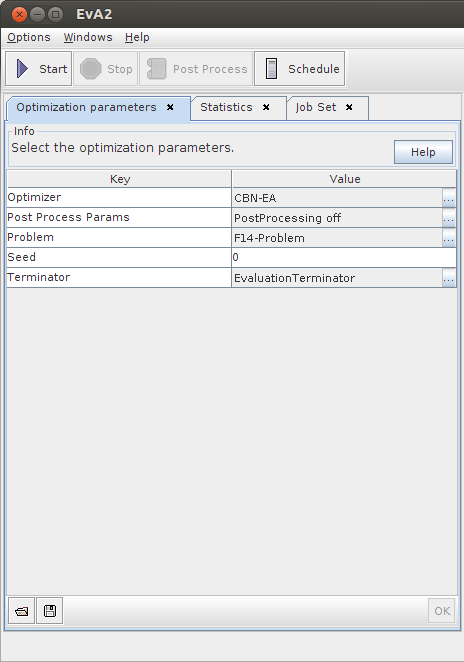
\includegraphics[width=0.45\textwidth]{pics/screenshot-workb-2013}~~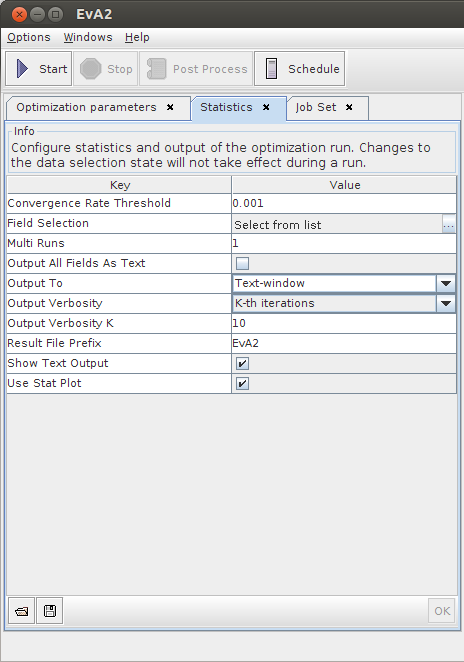
\includegraphics[width=0.45\textwidth]{pics/screenshot-stat-2013}
\par\end{centering}

\caption{Screenshots of the workbench window, with optimization (left) and
statistics (right) parameters.\label{fig:Screenshots-workbench}}
\end{figure}



\subsection{The Workbench Window\label{sub:The-Workbench-Window}}

The optimization parameters:
\begin{description}
\item [{\textit{Optimizer}}] Select the main optimization method. You can
choose between classical as well as evolutionary and swarm-based optimization
methods. For quick optimization, just use the standard values of the
parameters and try several different optimizers.
\item [{\textit{Post-processing~parameters}}] In some cases, post processing
of the results is desirable, e.g. if you want to improve the single
found solution by small hill climbing steps, or if you want to retrieve
more than one solution from a clustering optimization approach.
\item [{\textit{Problem}}] The instance of the target function to be optimized
is specified here. You can select from the benchmark problems delivered
with the package or inherit from the problem class yourself (Sec.~\ref{sec:Using-the-API}).
\item [{\textit{Random~Seed}}] As most algorithms in \noun{EvA2} incorporate
stochastic components, the random seed is critical for the specific
outcome of a run. For replicable results, set a seed value > 0. To
receive statistically relevant results, test several times with a
seed of 0, which means that the system time is used as seed for each
new run, or use the multi-run option.
\item [{\textit{Termination~Criterion}}] Set the criterion by which to
stop an optimization run, e.g. stop after \emph{n} fitness evaluations.
\end{description}
The Statistics parameters:
\begin{description}
\item [{\textit{Convergence~Rate~Threshold}}] Provided the target value
is zero, convergence is assumed if a value smaller than this threshold
is reached. For multi-run experiments, the number of hits is counted
using this criterion.
\item [{\textit{Field~Selection}}] The data fields to be displayed can
be selected. Typically, the current and best fitness are of most important,
but other fields such as average distance of candidate solutions may
be of interest. Since some data fields are complex types, such as
arrays, they are not plotted in the graph window but dumped to the
text window if marked. Depending on the problem and optimizer in use,
different data fields may be available. Specific information on the
data fields is given by tool tips in the application.
\item [{\textit{Number~of~Multi-runs}}] To achieve statistically meaningful
results on how well a certain optimizer works on a given problem,
set this number to do several runs in a row. The plot will be averaged,
while all intermediate data can be collected in an output file or
text window.
\item [{\textit{Output~All~Fields~As~Text}}] In some cases it is helpful
to show only selected data fields graphically but dump all data fields
to the text listeners, e.g., for external analysis.
\item [{\textit{Output~To}}] Textual information can be shown in a text
box, or redirected to a file, or both. The output file will be stored
to the current directory with a descriptive name containing the timestamp
of the start of the run.
\item [{\textit{Output~Verbosity}}] Select the verbosity of the textual
output, possible settings are ``no output'', ``final results'',
``k-th iterations'' and ``all iterations''. An iteration is usually
a generational cycle, meaning that for ``all iterations'', intermediate
data is printed after each generation.
\item [{\textit{Verbosity~Parameter~k}}] Define the interval parameter
for the ``k-th iterations'' setting of the output verbosity, by
which intermediate data is printed.
\end{description}
Finally, there are three buttons on top. \emph{``Description}''
shows some very general information on the main \noun{EvA} module.
The ``\emph{Start}'' button, as expected, starts an optimization
run using the parameters set, or multiple runs sequentially if \emph{multiRuns}
is set higher than one. During optimization, the ``\emph{Stop}''
button can abort the (multi-)run.


\subsection{The Plot Window}

\begin{figure}
\noindent \begin{centering}
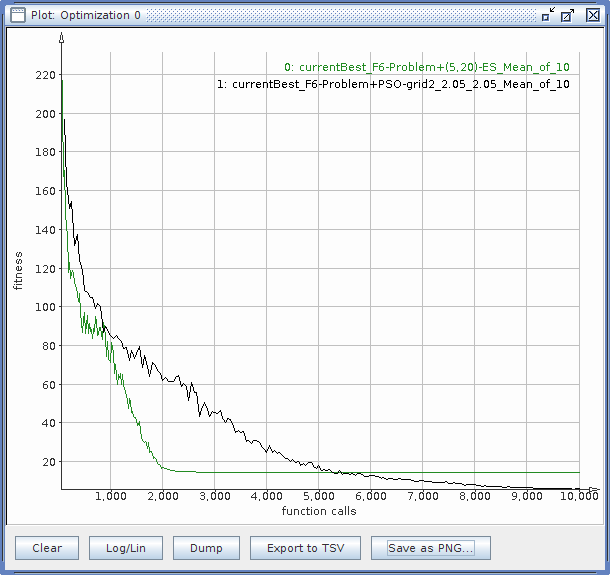
\includegraphics[width=0.52\textwidth]{pics/screenshot-plot-window}
\par\end{centering}

\caption{Plot window comparing a simple (5,20)-ES and PSO on Rastrigin's after
10 runs each.\label{fig:The-plot-window}}
\end{figure}


During the optimization run, the progress of the solution is plottet
to a graph in a separate window (Fig.~\ref{fig:The-plot-window}).
Usually, the fitness of the best individual of every generation is
drawn in Y-direction along the number of function calls in X-direction.
Be aware that for multi-objective problems, only the first fitness
dimension is shown. The 2-dimensional multi-objective problem classes
have, however, a pareto-front viewer which displays the population
in the two fitness dimensions sequentially. For higher fitness dimensions
it is more practical to use external tools for visualization. Figure~\ref{fig:The-plot-window},
by the way, shows the fitness progress averaged over 10 runs of a
(5,20)-ES and a PSO strategy on Rastrigin's Problem: PSO converges
slower, but finds better results on the long run, while ES settles
earlier on higher plateaus. 

The visible buttons have the following functions:
\begin{description}
\item [{\emph{Clear}}] Remove all graphs from the plot window.
\item [{\textit{Log/Lin}}] Switch between linear and log-scaled view. Most
benchmark problems in \noun{EvA} are implemented with the minimum
fitness at zero, so that the log-scale view allows to compare and
analyze convergence behaviour in detail. Of course, if the target
fitness may become zero or negative, log-scale view is impossible.
\item [{\textit{Dump}}] Export the contained data to standard output. For
each graph, a column is created in the same order they were generated.
\item [{\textit{Export}}] Create the same output as \textit{Dump} and save
it to a file.
\item [{\textit{Save}\noun{~}\textit{as}\noun{~}\textit{PNG}}] Create
a PNG image of the plot window and save it to a file.
\end{description}

\subsection{Basic Optimization using \noun{EvA2}\label{sub:Basic-Optimization-GUI}}

To get a grip on \noun{EvA2} and what optimization means, it is best
to run some experiments on the implemented standard benchmarks. To
do that, start the GUI and select a benchmark problem, e.g. the F1-Problem
consisting in a simple hyper-parabola. Leave the post-processing deactivated.
Then choose an optimizer, such as Evolution Strategies with standard
parameters, set the termination criterion to EvaluationTerminator
with 10,000 fitness calls and push the ``Start Optimization'' button
at the top of the window. Two additional windows will now open up:
the plot window with a fitness graph, and a text box displaying the
optimization progess in textual form. The final result will be printed
into the text box at the end of the run, as well.

If you play around with some optimizer settings, e.g. you try different
values for $\mu$ and $\lambda$ or activate the plusStrategy checkbox,
you will notice changing performance of the ES. On problems within
discrete space, such as the B1-benchmark problem, for example, a Genetic
Algorithm is often superior to an Evolution Strategy. You can try
this if you clear the plot window, select the B1-problem and run the
ES a few times. Now, switch to the Genetic Algorithm and run the optimization
a few more times.

Notice, however, that by changing from the F1-problem to the B1-problem,
the internal representation of individuals may change. As B1 is a
typical binary problem, it uses GAIndividuals by default, which are
based on binary vectors, while F1 uses double vectors. Be aware, that
not all optimizers in \noun{EvA2} are built to work on all types of
indviduals.


\subsection{Post-Processing\label{sub:Post-Processing}}

To see how post processing works, you can select the \emph{FM0Problem}
from the problem list, which is a simple target function with a global
and a local optimum. Select the \emph{ClusterBasedNiching} algorithm
as the optimizer. Now click on the \emph{postProcessingParams} and
activate them. For a clustering distance of $\sigma=0.1$ and $\approx5,000$
hill climbing steps, the optimizer should print out just a few solutions
in the text box, the first of which hopefully are the optima near
(1.7/0) and (-1.44/0).

Post-processing serves mainly two purposes: filter redundant solutions
and refine the search results. Redundant solutions occur naturally
in population-based heuristics. The optimizer handles several potential
solutions in parallel, and it is hoped that they all converge on the
global optimum during the run. Or for multi-modal problems which have
several local optima, it can be desirable to have parts of the population
converge in different areas of the solution space. In any case, one
usually wants to retrieve \emph{the} solution set or a refined global
optimum. For this purpose, we employ a clustering approach which takes
the whole solution set and merges similar solutions to an associated
subset. For each of these bulks, only the best individual is returned
in the filtered solution set. 

\begin{figure}
\noindent \begin{centering}
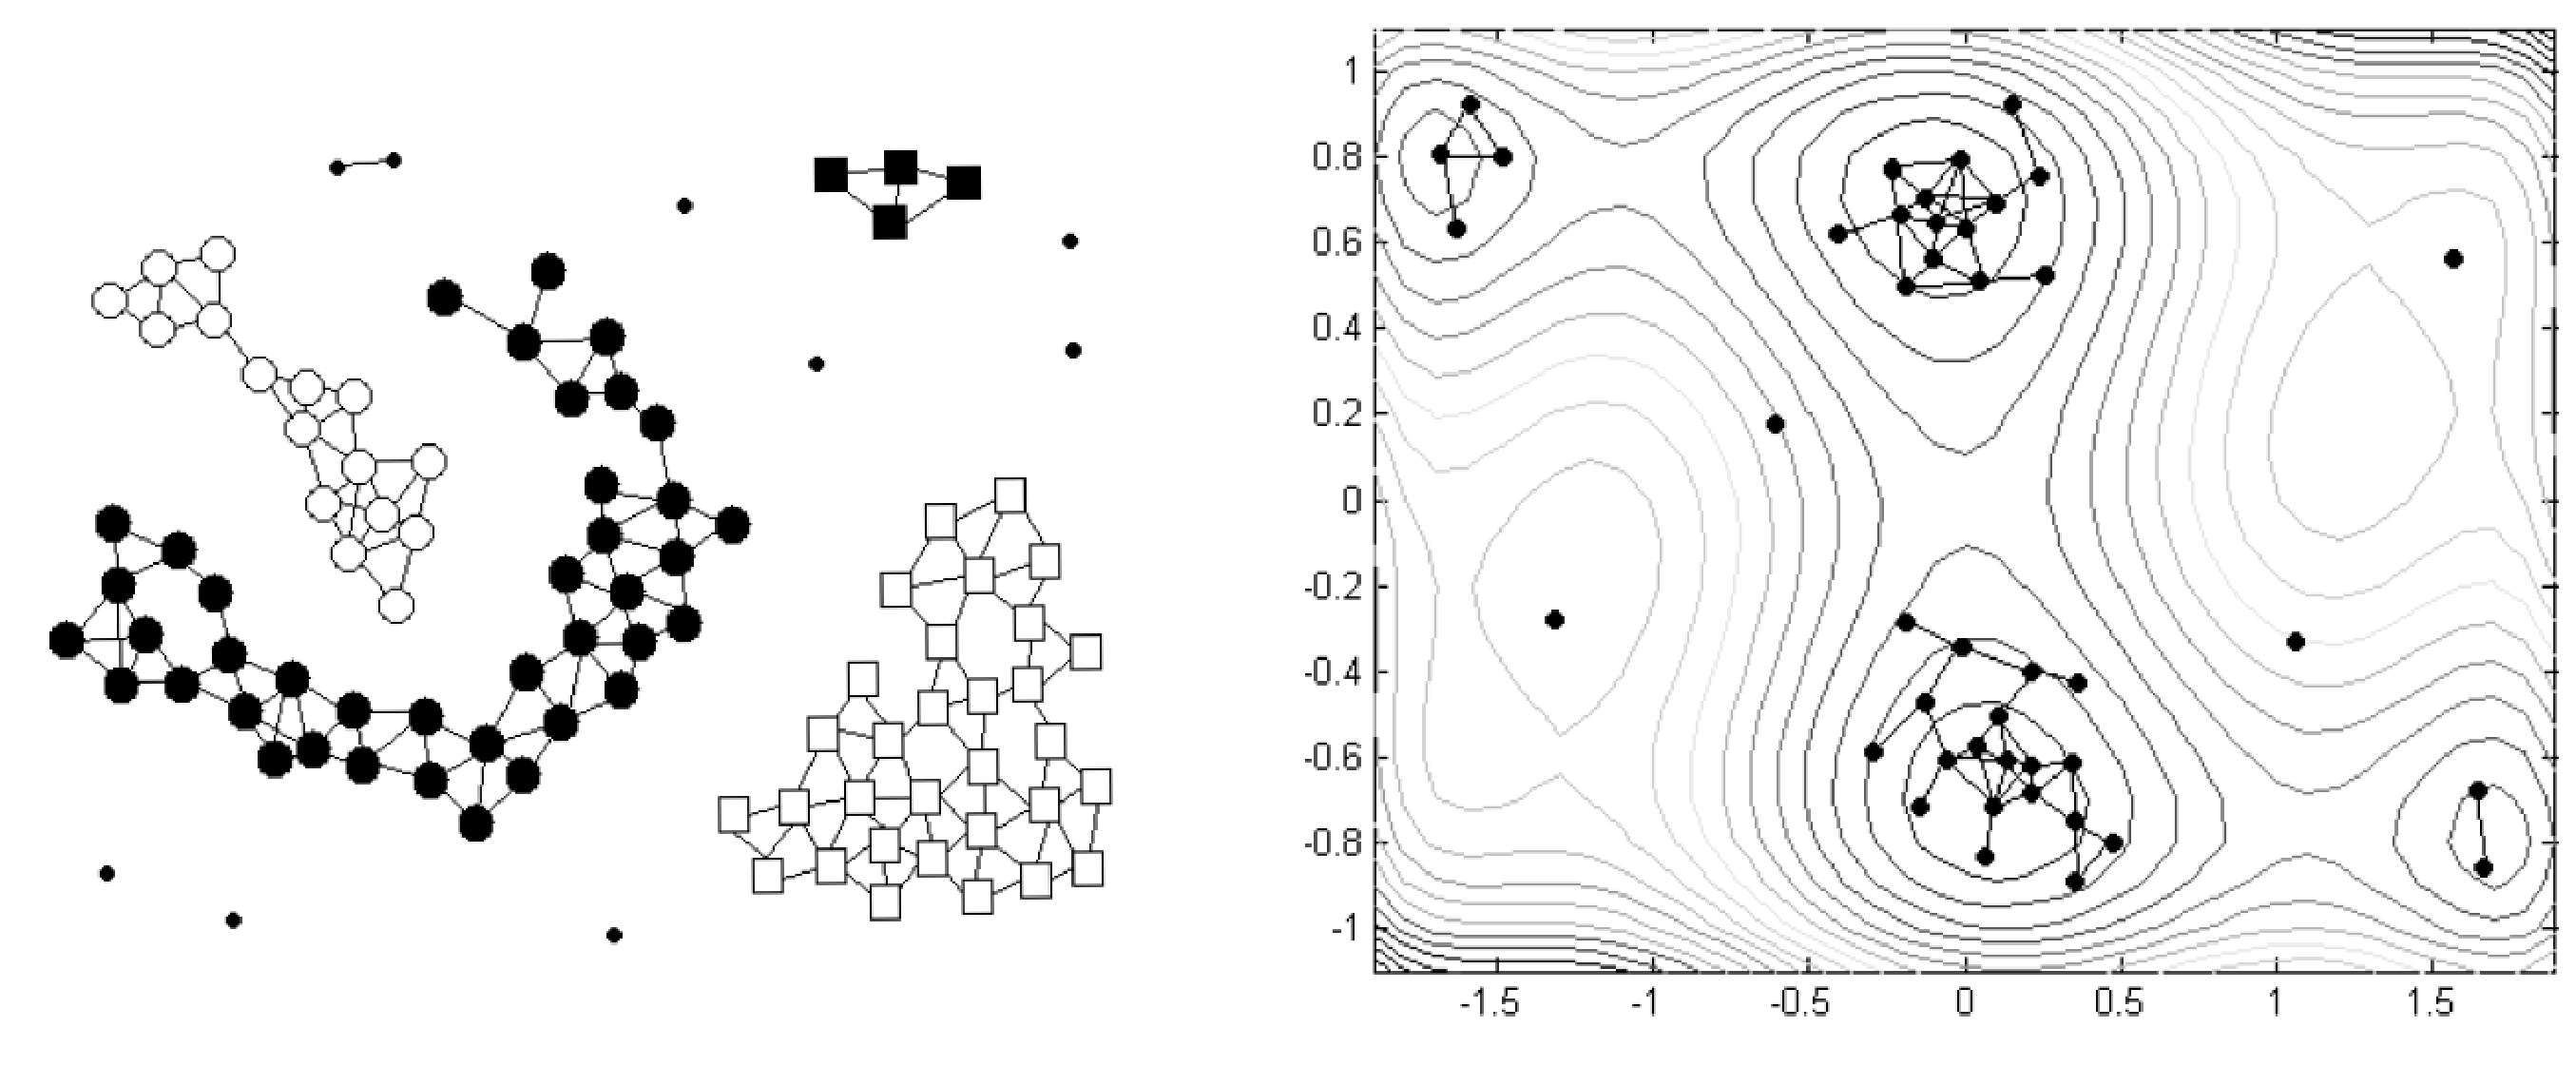
\includegraphics[width=0.8\columnwidth]{pics/cluster-graph}
\par\end{centering}

\caption{Examples for density based clustering (Streichert et al. \cite{streichertClustering03}).\label{fig:Density-based-clustering.}}
\end{figure}


Of course the size of this filtered set depends on the degree of convergence
in the original set and on the clustering criterion. We employ density
based clustering \cite{ester96density}, which associates any two
individuals which have a distance of less than the clustering parameter
$\sigma$ (Fig.~\ref{fig:Density-based-clustering.}). This is an
intuitive approach that does not require a predefined number of clusters,
in contrast to k-means, for example. By defining $\sigma$, you thus
define the resolution you grant your solution set.

As the solution set always contains the last state of the heuristic
optimization, one may hope that it is converged. But of course often
it is not fully converged, or maybe the strategy even rediversifies
the population from time to time, meaning that some part of the set
it is converged while other individuals are freshly initialized and
thus by no means optimal. So after filtering out redundancy, you might
also want to refine the returned set a little. This can be done directly
by Hill Climbing (HC) in the post-processing step by setting \emph{postProcessSteps}
to the number of evaluation calls you want to invest in the refinement.%
\begin{comment}
Question here: what is a hill climber?
\end{comment}


If you set $\sigma$ for clustering and performed hill climbing, then
there will be another clustering step right after the HC process,
to remove redundancy that emerged by the additional HC optimization.


\section{Additional Packages}

To add additional packages to use them with the \noun{EvA2} base package,
you can just add them to the class path. For instance, to use the
additional ``Probs'' package containing a larger set of benchmark
problems, place them both in your working directory and type (GNU/Linux):
\begin{quotation}
\texttt{\small \$ java -cp EvA2.jar:EvA2Probs.jar eva2.gui.Main}{\small \par}
\end{quotation}
You should now be able to select from a larger set of optimization
problems in the GUI. Note that different platforms use different characters
as path separators (':' in GNU/Linux). To add your own classes to
the \noun{EvA2} framework (see Sec.~\ref{sec:Quickly-Adding-Your-Problem}),
you need to add your local development path to the classpath, for
example:
\begin{quotation}
\texttt{\small \$ java -cp EvA2.jar:EvA2Probs.jar:/home/username/OwnClassDir
\textbackslash{}}{\small \par}

\texttt{\small eva2.gui.Main}{\small \par}
\end{quotation}
Note that \noun{EvA2} will search all classpath entries for compatible
classes, so you should only add those packages which are really required.
For your own additional packages, this also means that, if you want
your extensions (e.g. own problem implementations or operators) to
be displayed in the \noun{EvA~2} GUI, they have to be assigned the
same package tree as the associated \noun{EvA2} operators. Check Sec.~\ref{sec:Using-the-API}
on more details.

\include{chapters/03-external-interface}
\chapter{Quickly Adding a Problem Class\label{sec:Quickly-Adding-Your-Problem}}

It is easy to integrate your own Java-coded problem in \noun{EvA2}
and optimize it using the GUI. Preconditions for the quick way are
only the two following ones:
\begin{itemize}
\item A potential solution to your problem can be coded as a double vector
or a BitSet.
\item You can implement the target function such that it produces a double
valued fitness vector from the double vector or BitSet.
\end{itemize}
If these simple conditions are met, you have the advantage of being
able to use the full ``Java-Power'' to implement a target function
and optimize it in \noun{EvA2}. Just follow these steps:
\begin{itemize}
\item Create an empty class (let's say, \texttt{ExampleProblem}) and assign
it to the package \texttt{eva2.problems.simple}. Put it in a directory called
``eva2/problems/simple/'' within your working directory.
\item Have the class inherit from \texttt{eva2.problems.simple.SimpleDoubleProblem}
or, depending on which datatype you want to use, from \texttt{eva2.problems.simple.Simple\-Binary\-Problem}.
Both base types can be used directly from the \noun{EvA2} jar-file
(which of course needs to be on the java classpath - in Eclipse, for
instance, add the \noun{EvA2} jar as ``External jar'' to the Java
build path through the project settings).
\item Implement the method \texttt{public int getProblemDimension() \{...\}}
whithin your ExampleProblem, which returns the number of dimensions
of the solution space, i.e. the length of the \emph{x} vector or size
of the \texttt{BitSet}, respectively. The problem dimension may be
a variable defined in your class, but it must not change during an
optimization run.
\item Implement the method \texttt{public double{[}{]}} \texttt{evaluate(double{[}{]}
x)} for double coded problems or \texttt{public} \texttt{double{[}{]}}
\texttt{evaluate(BitSet} \texttt{bs)} for binary coded problems, whithin
your ExampleProblem, where the fitness of a potential solution is
calculated.
\item Start the \noun{EvA2} GUI. \emph{Make sure that your working directory
is in the Java classpath}! From the problem list, select the \emph{SimpleProblemWrapper}
class as optimization problem. The wrapper class allows you to select
your ExampleProblem as target function. If you implemented a double
valued problem, you may also set a default range parameter, defining
the positive and negative bound of the solution space allowed. Now
select your prefered optimization method and start the optimization.
\end{itemize}
\chapter{Using the EvA2 API\label{sec:Using-the-API}}

This chapter describes how to incorporate \noun{EvA2} into existing
projects through the Java API.


\section{Accessing Standard Optimizers\label{sub:Accessing-Standard-Optimizers}}

A standard optimizer is typically a well-known optimization algorithm
with operators and parameters predefined in a way so that a user may
start it out-of-the-box and expect good optimization results in general.
Of course, every expert may have an own notion on what parameters
are preferable in general. Therefore we give two customization examples
using the API. In any case, a necessary step is to extend a \noun{EvA2}
base class constituting the target function. You may, again, use the
\texttt{eva2.problems.simple} package described in Sec.~\ref{sec:Quickly-Adding-Your-Problem}.
However, this makes it necessary to use the wrapper class \texttt{SimpleProblemWrapper},
which is great for direct GUI usage but may make programming a bit
more complicated. We therefore, at this point, recommend to go one
step higher in hierarchy and extend \texttt{AbstractProblemDouble}
or \texttt{AbstractProblemBinary}.


\subsection{The Abstract Problem Classes\label{sub:The-Abstract-Problem-classes}}

The problem class subtree encapsulates properties of target functions
that can be directly optimized by the \noun{EvA2} framework and starts
at the \texttt{AbstractOptimizationProblem} class. The basic properties
of the problem class are functional: 
\begin{enumerate}
\item The problem is itself initialized, 
\item the problem knows how to initialize a set of potential solutions,
and 
\item the problem evaluates a set of potential solutions. 
\end{enumerate}
To implement your own target function in \noun{EvA2}, we recommend
inheriting from \texttt{AbstractProblemDouble} or \texttt{AbstractProblemBinary},
depending on your preferred data representation. Integer and program-data-based
problems are currently not covered by this document. Notice that if
you want your problem implementation to be displayed and manageable
by the GUI in the same way the predefined problems are handled, you
have to assign it the same package tree as its parent class (e.g.
\texttt{eva2.problems} for new problem implementations).


\paragraph*{The class \texttt{AbstractProblemDouble}}

The \texttt{AbstractProblemDouble} class in the package \texttt{eva2.prob\-lems}
encapsulates methods useful to implement double valued target functions.
Let's assume you want to implement a function $f_{\mathrm{target}}(x)=y$
with $f_{\mathrm{target}}:\;\mathbb{R}^{n}\rightarrow\mathbb{R}^{m}$.
Important for double-valued problems is the range of the solution
space, defining in any dimension the minimum and maximum value allowed.
By setting the \texttt{default\-Range} member variable (method \texttt{set\-Default\-Range})
in your constructor, you can easily define a symmetric range $[-dR,\; dR]^{n}$.
If you need a different range definition, you may overload the methods
\texttt{getRangeLowerBound(int dim)} and \texttt{getRangeUpperBound(int
dim)} which are to return the upper or lower range limit for a given
dimension.%
\begin{comment}
template? noise?
\end{comment}
{} 

The \texttt{AbstractProblemDouble} class also contains a noise parameter
and an individual template. The \emph{noise} can be used to add gaussian
fluctuation to any target function. If \emph{noise} > 0, it defines
the standard deviation of the random disturbance of $f_{\mathrm{target}}(x)$.
The individual template defines the data representation for potential
solutions. It also contains evolutionary operators which work directly
on the representation, see Sec.~\ref{sub:Setting-Evolutionary-Operators}
for a usage example.

We will now give short comments on further important member functions:
\begin{description}
\item [{\texttt{public ~Object ~clone()}}] Object copy operator. We recommend
implementing a copy constructor \texttt{public YourProblem(YourProblem
o)} and refering to it from within the \texttt{clone()} method. You
may call \texttt{cloneObjects} from AbstractProblemDouble to copy
the super members. Make sure that the copy constructor copies all
necessary member variables you added to your class.
\item [{\texttt{public ~void ~evaluate(AbstractEAIndividual ~individual)}}] Main
evaluation method. We recommend not to override it.
\item [{\texttt{public ~abstract ~double{[}{]} ~evaluate(double{[}{]} ~x)}}] Essential
evaluation method. Override it to implement the desired target function
$f_{target}(x)$. Make sure that the delivered solution vector is
always of the same dimensionality $m$. Even if your problem is one-dimensional,
return an array of length 1 with the single fitness value as the only
field.
\item [{\texttt{public ~abstract ~int ~getProblemDimension()}}] Return
the problem dimension in solution space. Make sure it is constantly
equal to $n$ during an optimization run. If you implement a corresponding
method \texttt{public void setProblemDimension(int n)} and define
your class within the same package, you may change the dimension through
the GUI.
\item [{\texttt{public ~void ~initializeProblem()}}] Called before optimization
in general. If you define member variables of your class which are
not constant, we recommend setting them to initial values in this
function. If you override, make sure you call the super-method from
within your version.
\item [{\texttt{public ~void ~initializePopulation(Population ~population)}}] This
method is called before optimization with a certain population. It
initializes the population to the problem specific range using the
individual template and calls a method of the \texttt{Population}
collection to initialize the individuals randomly whithin the range.
If you want to alter the way the individuals are initialized, we recommend
overriding this method. Call the super-method from your implementation
and make changes to the individuals afterwards.
\end{description}
For an example on how to extend \texttt{AbstractProblemDouble} you
can look at the \texttt{F1Problem} class which implements a simple
parabola function.


\paragraph*{The class \texttt{AbstractProblemBinary}}

The binary variant is widely analogous to \texttt{AbstractProblemDouble}.
The main differences are that there is no range definition (the range
is always $0^{n}-1^{n}$) and that the template is of a different
type, namely \texttt{GAIndividualBinaryData}, and delivers a Java
\texttt{BitSet} as data representation instead of a double vector.
The \texttt{eval} function signature changes accordingly, and to implement
a target function $g_{\mathrm{target}}(x)=y$ with $g_{\mathrm{target}}:\;\{0,1\}^{n}\rightarrow R^{m}$,
you need to work on a \texttt{BitSet}%
\footnote{Concerning \texttt{BitSet}: it may be valuable to note that when looping
over a \texttt{BitSet}, it is preferable to use the self defined problem
dimension as index limit instead of \texttt{size()} or \texttt{length()}
methods of \texttt{BitSet}.%
} object.
%
\begin{description}
	\item [{\texttt{public ~abstract ~double{[}{]} ~evaluate(BitSet ~bs)}}] Essential
evaluation method. Override it to implement the desired target function
$g_{\mathrm{target}}(b)$. Make sure that the delivered solution vector
is always of the same dimensionality $m$. Even if your problem is
only one-dimensional, return an array of length 1 with the single
fitness value as only field.
\end{description}
%
For an example on how to implement binary functions, look at the \texttt{B1Problem}
class which realizes a simple minimize bits problem.


\subsection{The OptimizerFactory} \label{sub:The-OptimizerFactory}

To access default optimization algorithms easily, we have defined
an \texttt{OptimizerFactory} class. It allows to specify an optimization
algorithm by an ID number and mainly takes a problem class and an
optional output file as input. For example, if you have a double-valued
problem class and just want to retrieve one solution, use the \texttt{optimizeToDouble(final
int optType, AbstractOptimizationProblem problem, String outputFilePrefix)}
method, which returns the solution as a double vector. 

Table \ref{tab:Overview-OptimizerFactory} gives an overview over
the currently accessible optimization strategies. You may use \texttt{showOptimizers()}
to get a string with a summary of the implemented algorithms with
ID associations. A short example is shown in Listing \ref{alg:OptFact-Usage-example},
where PSO is used to optimize the simple hyper parabola (in 10 dimensions
by default). The PSO with $50,000$ evaluations should find a solution
very close to zero, e.g. absolutely below $10^{-30}{}{}$ in every
dimension.

\begin{algorithm}
\lstinputlisting[style=myjavastyle]{../../src/eva2/examples/TestingF1PSO.java}

%\begin{algorithmic}  \IF {$i\geq maxval$}          \STATE $i\gets 0$ \ELSE         \IF {$i+k\leq maxval$}                 
%\STATE $i\gets i+k$          \ENDIF \ENDIF  \end{algorithmic}

\caption{Simple \texttt{OptimizerFactory} usage example.\label{alg:OptFact-Usage-example}}
\end{algorithm}


\begin{table}
\begin{tabular}{|l|l|}
\hline 
ID & Short Description\tabularnewline
\hline 
\hline 
STD\_ES & A standard (15,50)-Evolution Strategy.\tabularnewline
CMA\_ES & (15,50)-Evolution Strategy with Covariance Matrix Adaptation.\tabularnewline
STD\_GA & Standard Genetic Algorithm with elitism\tabularnewline
PSO & Particle Swarm Optimization with constriction.\tabularnewline
DE & Differential Evolution\tabularnewline
TRIBES & Tribes: an adaptive PSO\tabularnewline
RANDOM & Random search (Monte-Carlo)\tabularnewline
HILLCL & Multi-start hill climbing\tabularnewline
CL\_HILLCL & Clustering multi-start hill climbing\tabularnewline
CBN\_ES & Clustering-based Niching ES\tabularnewline
\hline 
\end{tabular}

\caption{Overview over algorithms accessible through OptimizerFactory.\label{tab:Overview-OptimizerFactory}}
\end{table}



\section{Termination Criteria\label{sub:Termination-Criteria}}

To configure the termination criteria of an optimization process started
through the OptimizerFactory, use the setTerminator family. The default
terminator stops at a maximal number of fitness evaluations, e.g.
$10,000$. To change the number of evaluations performed to, for example,
$50,000$, call \texttt{Optim\-izer\-Fac\-tory.set\-Evaluation\-Ter\-mi\-na\-tor(50000)}
before starting the optimization, as in Alg.~\ref{alg:OptFact-Usage-example}.

For more flexible termination criteria, there are several Terminator
parameter classes you can use and set them directly using \texttt{Optim\-izer\-Fac\-tory.set\-Ter\-mi\-na\-tor(term)}.
Available are the following variants:
\begin{lyxlist}{00.00.0000}
\item [{\texttt{EvaluationTerminator}:}] Construct with a maximal number
of evaluations. Parameters: 

\begin{lyxlist}{00.00.0000}
\item [{\texttt{maxEval}:}] integer number of evaluations to be performed
at maximum.
\end{lyxlist}
\item [{\texttt{GenerationTerminator}:}] Terminate after a given number
of generations. As not all algorithms use constant population sizes,
we suggest to use EvaluationTerminator preferably. Parameters: 

\begin{lyxlist}{00.00.0000}
\item [{\texttt{gens}:}] integer number of generations to be performed
at maximum.
\end{lyxlist}
\item [{\texttt{FitnessValueTerminator}:}] A minimum fitness value (vector)
must be reached to terminate. Construct with a double array representing
the target fitness value. Parameters: 

\begin{lyxlist}{00.00.0000}
\item [{\texttt{v}:}] double array fitness vector to be reached.
\end{lyxlist}
\item [{\texttt{CombinedTerminator}:}] For effective optimization, one
might want to combine several criteria in a boolean way, i.e. terminate
if $20,000$ evaluations have been performed OR the best fitness doesn't
change for $1,000$ evaluations. To allow for this, we provide the
\texttt{CombinedTerminator} class which just takes to terminator instances
and combines them logically. Thus, terminators can be nested as required.
Parameters:

\begin{lyxlist}{00.00.0000}
\item [{\texttt{t1}:}] First terminator to combine.
\item [{\texttt{t2}:}] Second terminator to combine.
\item [{\texttt{logicalOperator}:}] Flag indicating whether to use conjunctive
AND or disjunctive OR combination.
\end{lyxlist}
\end{lyxlist}
\begin{lyxlist}{00.00.0000}
\item [{\texttt{MaximumTimeTerminator}:}] Terminate after a maximum time has been reached: 

\begin{lyxlist}{00.00.0000}
\item [{\texttt{maxTime}:}] integer number of seconds
at maximum.
\end{lyxlist}
\end{lyxlist}
A specific class of terminators checks for convergence of a population
measure, such as the average distance of individuals within the population.
Common to these terminators is the required definition of convergence.
Generally, convergence is assumed if the measure $m(P(t))$ has not
changed more than a certain threshold $\theta$ during a fixed time
period $t_{S}$. The stagnation time $t_{S}$ may either be taken
as fitness calls (calls to the target function) or generations (iterations
of the optimizer), however the population measure is calculated only
after full generations.

The convergence threshold may either be an absolute value, a change
of the absolute value compared to $m(P(t-t_{S}))$ or a change of
the relative ratio of the value $m(P(t-t_{S}))$. Additionally, stagnation
may be determined if no decrease by more than \texttt{$\theta$} has
occurred, or if no change occured (bidirectional: neither decrease
nor increase by more than \texttt{$\theta$}). In the case of bidirectional
check, termination occurs if the population measure changes less than
\emph{$\theta$} for the stagnation period \emph{$t_{S}$}: $\forall\, i\in\{0,1,...p-1\}:m(x_{t-t_{S}})-\delta\le m(x_{t-i})\le m(x_{t-t_{S}})+\delta$,
where $m(x_{t})$ stands for the population measure of individual
$x$ at generation $t$. The allowed boundary $\delta$ is given with
the fixed threshold in the absolute change case ($\delta=\theta$)
or calculated from $m(x_{t-t_{S}})$ in the relative change case:
$\delta=\theta\cdot m(x_{t-t_{S}})$. In the absolute value case,
$m(x_{t-i})$ is directly compared to $\theta$: $m(x_{t-i})\leq\theta$
must hold for $t_{S}$ iterations.

The following Terminators are based on this convergence criterion:
\begin{lyxlist}{00.00.0000}
\item [{\texttt{FitnessConvergenceTerminator}:}] Terminate as soon as there
is hardly any improvement (or change) in the fitness of the best individual
for a certain period of time. In a multi-objective case, the 2-norm
of the fitness vector is calculated (however a pareto metric should
be prefered in these cases). Parameters: 

\begin{lyxlist}{00.00.0000}
\item [{\texttt{checkType}:}] check for decrease only of the measure or
bidirectional change, where the measure may not leave in both directions
to determine stagnation.
\item [{\texttt{convergenceCondition}:}] check for relative change, absolute
change or absolute value reached along the stagnation time.
\item [{\texttt{convergenceThreshold}:}] double valued fitness threshold
\emph{$\theta$.}
\item [{\texttt{stagnationMeasure}:}] interprete the stagnation time as
number of function calls or generations.
\item [{\texttt{stagnationTime}:}] integer length of the stagnation time.
\end{lyxlist}
\item [{\texttt{PhenotypeConvergenceTerminator}:}] In analogy to the \texttt{FitnessConvergenceTerminator},
terminate as soon as there is hardly any change in the best phenotype,
meaning that $m(P)=x_{best}$ for the best indiviual $x_{best}\in P(t)$.
Parameters: see \texttt{FitnessConvergenceTerminator}.
\item [{\texttt{DiversityTerminator}:}] Terminate as soon as the average/minimal/maximal
distance of individuals in the population stagnates. Thus, $m(P)$
calculates distances on all individuals in $P$ at every iteration,
which may be time-consuming. Parameters: see \texttt{FitnessConvergenceTerminator},
with additions:

\begin{lyxlist}{00.00.0000}
\item [{\texttt{criterion}:}] Check the minimal, maximal or average distance
as diversity measure on $P$.
\item [{\texttt{metric}:}] The metric to use for distance calculation.
\end{lyxlist}
\item [{\texttt{ParetoMetricTerminator:}}] Terminate if the Pareto front
of a multi-objective optimization problem stagnates. To measure progress
on pareto fronts, several metrics can be used. Note that this only
works with multi-objective problem instances. Parameters: see \texttt{FitnessConvergenceTerminator},
with additions:

\begin{lyxlist}{00.00.0000}
\item [{\texttt{paretoMetric}:}] The metric to use to measure change of
the Pareto front.
\item [{\texttt{useCurrentPop}:}] Apply the measure to the current population
or the current Pareto front stored by the optimizer.
\end{lyxlist}
\end{lyxlist}
Some notes on terminators: 
\begin{itemize}
\item Note that the termination criterion is always checked after one iteration,
i.e. one generation. This means that, if the number of evaluations
is not a multiple of the population size or the population size is
variable, the maximum number of evaluations may be slightly exceeded.
The same holds for the stagnation time in convergence terminators.
\item Concerning convergence terminators: Note that for flat plateaus in
fitness space, the fitness may hardly change while there is still
progress in the solution space. On the other hand, note that highly
nonlinear problems may hardly change in phenotype but still change
considerably in fitness. When using convergence terminators, we suggest
to set the stagnation period sufficiently high. Also, take care when
checking for relative convergence with measures tending towards zero,
since relative fluctuations with very small values may be high without
showing real progress.
\end{itemize}
For a usage example that creates and sets a terminator which stops
if either $20,000$ evaluations have been performed or both best fitness
and phenotype stagnate for $1,000$ evaluations, see Listing~\ref{alg:Comb-terminator}.
Note that ``convergence'' in this context refers to stagnation After
a combined termination, one might want to know why the run actually
stopped. The method \texttt{terminatedBecause()} implemented in \texttt{OptimizerFactory}
as well as any terminator object will return a String object describing
the exact reason, while the method \texttt{lastEvalsPerformed()} informs
on how many evaluations were required. The PSO in the given example
should require about $5,000-7,000$ evaluations to meet the two convergence
criteria.

\begin{algorithm}


\lstinputlisting[style=myjavastyle]{../../src/eva2/examples/TerminatorExample.java}

\caption{Terminator combination example.\label{alg:Comb-terminator}}
\end{algorithm}



\section{Customizing the Optimization}

Beyond standard optimizers, you may wish to customize optimization
parameters manually or iterate over different settings in a loop.
To do this, you need to access the optimization parameter structure
\texttt{OptimizationParameters} and alter its values before starting optimization.
A \texttt{OptimizationParameters} instance contains all settings required for
an optimization run: target function, optimizer, random seed, post-processing
options and termination criterion; basically all that is also set
through the workbench window of the GUI (Sec.~\ref{sub:The-Workbench-Window}).
To alter specific settings, it is sufficient to alter a \texttt{OptimizationParameters}
instance generated by the \texttt{OptimizerFactory} and then start
the optimization using this altered parameter instance.


\subsection{Accessing Parameters}

Look at Listing \ref{alg:Customizing-optimization.} for an example
on how to customize optimization parameters. To find out about which
operators are implemented and usable, it is again easiest to check
out in the GUI, where there are also short descriptions available.

\begin{algorithm}
\lstinputlisting[style=myjavastyle]{../../src/eva2/examples/TestingGAB1.java}

\caption{Customized optimization example.\label{alg:Customizing-optimization.}}
\end{algorithm}


Note that in example \ref{alg:Customizing-optimization.}, there will
actually be $1,050$ evaluations performed, which is the first multiple
of the population size of 150 that exceeds the maximum evaluation
limit of $1,000$ set. To change the population size before a run,
simply set a new population of the target size. Any population will
be initialized to contain the given number of individuals by the problem
class, usually in a random distribution over the problem range.


\subsection{Setting Evolutionary Operators\label{sub:Setting-Evolutionary-Operators}}

\begin{algorithm}
\lstinputlisting[style=myjavastyle]{../../src/eva2/examples/TestingPlusCmaEs.java}

\caption{Setting up a (1+5) CMA-ES.\label{alg:(1+5)-CMA-ES.}}
\end{algorithm}


In Listing~\ref{alg:(1+5)-CMA-ES.}, a (1+5) CMA-ES is configured
and run on a simple bimodal target function with the global optimum
near (1.7/0) and a local one near (-1.44/0). The (1+5)-CMA-ES is powerful
and will find the global optimum most of the time. Sometimes, however,
due to its relatively high selection pressure and elitistic strategy,
it will converge in the local optimum, depending on the random initialization.

Lines 23-26 of Listing~\ref{alg:(1+5)-CMA-ES.} show how to access
evolutionary operators directly. What happens here is that the template
individual delivered with the problem class (because the problem defines
the representation) is modified to use the given mutation and crossover
operator and probabilities. Typical for ES, the mutation probability
$p_{m}$ is relatively high, while the crossover probability $p_{C}$
is rather low. One could also use \texttt{fm0.get\-Individual\-Template().set\-Mutation\-Operator(...)}
etc. to set the operators and probabilities one by one just as through
the GUI. Notice that not all implemented heuristics make use of individual
evolutionary operators. Several come with their own operator definitions,
such as DE and PSO, for example. The Hill Climbers, on the other hand,
do use individual mutation but override individual probabilities to
$p_{m}=1$ and $p_{c}=0$ by definition.


\subsection{A Multi-Modal Example with Post-Processing\label{sub:A-Multi-Modal-Example}}

When looking at the last example in \ref{sub:Setting-Evolutionary-Operators}
working on a bimodal function, one might ask how to retrieve more
than just one optimum of the target function. In \noun{EvA2} there
are some optimizers implemented which are specialized on this task.
Listing~\ref{alg:CBN-pp} shows an example using the clustering-based
niching EA (CBN-EA) \cite{streichertClustering03} and post-processing
to identify both optima of the target function.

\begin{algorithm}
\lstinputlisting[style=myjavastyle]{../../src/eva2/examples/TestingCbnPostProc.java}

\caption{Solving a bimodal function with CBN and post-processing.\label{alg:CBN-pp}}
\end{algorithm}


Notice that two post-processing cycles are performed (lines 26 and
33). Any repeated post-processing iteration performed on the \texttt{OptimizerFactory}
uses the same initial state. This means that if there is no new optimization
cycle, any new post-processing will work on the same set of solutions,
namely the result population of the last optimization.

This is useful, for example, to search for optima using different
resolutions iteratively. In our example, we however just demonstrate
the different results without (line 26) and with clustering (line
33). If you run the example a few times, it will happen quite often
that after the first post-processing with clustering only, more than
the two optima are returned, while after the second step with hill
climbing, this will happen rather seldomly. All in all, CBN locates
the two optima in most of the cases and post-processing helps to identify
the real hot spot. In Fig.~\ref{fig:Exemplary-states-of-CBN}, two
graphs show the target function and the states of an exemplary CBN-run
after 500 (left) and 1,500 evaluations (right).

\begin{figure}
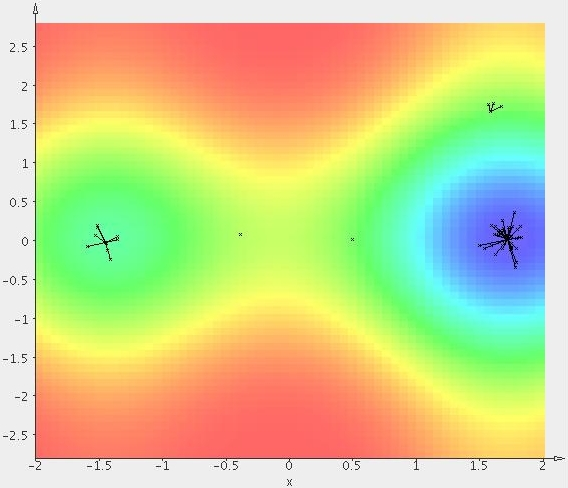
\includegraphics[width=0.49\columnwidth]{pics/fm0-cbn-500}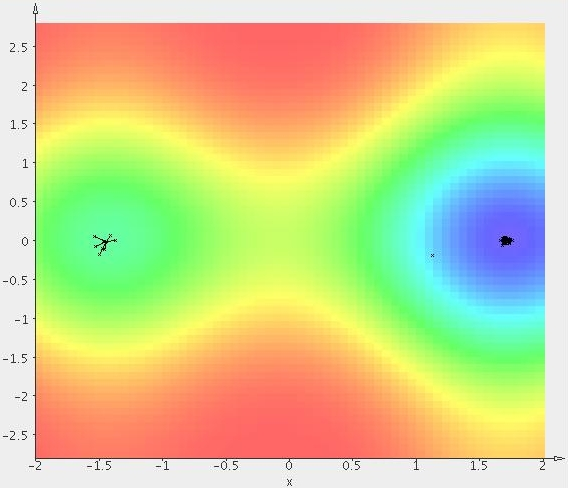
\includegraphics[width=0.49\columnwidth]{pics/fm0-cbn-1500}

\caption{Exemplary states of CBN on the simple bimodal FM0Problem.\label{fig:Exemplary-states-of-CBN}}
\end{figure}


The FM0Problem is of course very simple, 2-dimensional and having
only two optima in the defined range. For harder problems, a few thousand
evaluations will not suffice, and for highly multi-modal target functions,
e.g. if there are thousands or tens of thousands of local optima,
things get really tough. The current implementation of CBN is able
to find more optima than the population size defined, because it is
able to reinitialize a converged cluster during a run, saving a representative
to an archive. But for problems with a lot of deceptive optima, it
might also be a good strategy to concentrate on finding one global
optimum, and, as it won't be found in most of the runs, look at the
results of the single-run solution set.
\chapter{Further Reading\label{sec:Further-Reading}}

As noted before, this introduction does not cover algorithmic basics.
We recommend the introduction of Engelbrecht \cite{Engelbrecht07CI}
for newer strategies (DE, PSO) and Bäck et al. \cite{Baeck99EC1}
for classical Evolutionary Algorithms. The applications note from
2010 gives some short and simple use cases for the framework \cite{Kron10EvA2}.
To go into details of\noun{ }EvA2, a look on the technical report
of 2005 \cite{JOptDocumentation}, though slightly outdated, will
still be helpful, as well as the thesis of Felix Streichert \cite{Streichert07},
one of the main authors of \noun{JavaEvA}.


\begin{comment}

\chapter{General Hints on Optimization with \noun{EvA2}}

As you have come so far, you have hopefully learned a few things about
the concepts of \noun{EvA~2 }and got an idea on how optimization
in the framework can be done. Now we want to give a few more practical
hints on what to do with an unknown, probably difficult function.
Let's suppose you have a mathematical or algorithmic problem which
is infeasible to solve by means of mathematical analysis, gradients
are not computable in a simple way, and you haven't found a specialized
algorithm or heuristic in literature that solves it to the quality
you need, or you have found one but you don't understand it and can't
download it anywhere. All in all, you have a tough problem, \noun{MyToughProblem},
and you want to optimize it.

Let's also suppose you can implement \noun{MyToughProblem} in Java
(Sec.~\ref{sec:Quickly-Adding-Your-Problem}) or make it accessible
for\noun{ EvA~2} through an external interface (Sec.~\ref{sec:External-Interfaces}). 

You might now be tempted to ask: ``Exactly which optimizer do I need
to run with which parameters to solve \noun{MyToughProblem} once and
for all times?''.

And as you might have feared, this is a question which we cannot answer,
and maybe noone else can. But we will at least try to come a bit closer
to an answer here. There are several choices you have to make before
optimization, one of the earliest concern implementation: which representation
to use? E.g. in Sec.~\ref{sub:Accessing-Standard-Optimizers}, we
said a few things about double-valued and binary representation, and
many problems are natural to the one or the other implementation.
Combinatorical problems, for example, can be much easier projected
to a binary vector than to a double-valued one. Continuous functions
are a typical case for a real valued representation.
\begin{itemize}
\item which representation? 
\item how many optima? 
\item what range? 
\item will specialized operators help?
\item what about constraints?
\item what about multi objectives?
\end{itemize}
read the examples given in Sec.~\ref{sec:Using-the-API}, you might
So, for an unknown function

However, if you are dealing with an unknown function and you reckon
that it has quite a lot of optima, 
\begin{itemize}
\item Which options can be changed at all for optimizer X? -> anhang with
GOParameter classes? Some optimizers have no specialized GOParameters.
Access optimizer directly.
\end{itemize}

\chapter{Optimization Context}


\chapter{Architecture}


\section{The JE2 Modules}


\section{The Concepts}


\section{The GUI Workbench}


\section{The Configuration File}


\chapter{Advanced Use Cases}
\end{comment}


\bibliographystyle{plain}
\bibliography{EvA2DocCitations}

\end{document}
